\documentclass[10pt,twocolumn,letterpaper]{article}
\usepackage{cvpr}
\usepackage{times}
\usepackage{epsfig}
\usepackage{graphicx}
\usepackage{amsmath}
\usepackage{amssymb}
\usepackage[T1]{fontenc}
\usepackage{textcomp}
\usepackage{xcolor}
\usepackage{listings}
\definecolor{codegreen}{rgb}{0,0.6,0}
\definecolor{codegray}{rgb}{0.5,0.5,0.5}
\definecolor{codepurple}{rgb}{0.58,0,0.82}
\definecolor{backcolour}{rgb}{0.95,0.95,0.92}
\lstset{
  backgroundcolor=\color{backcolour},
  commentstyle=\color{codegreen},
  keywordstyle=\color{magenta},
  numberstyle=\tiny\color{codegray},
  stringstyle=\color{codepurple},
  basicstyle=\ttfamily\small,
  breaklines=true,
  breakatwhitespace=true,
  keepspaces=true,
  showstringspaces=false,
  frame=single,
  tabsize=4,
  columns=fullflexible,
  upquote=true
}

\usepackage[pagebackref=true,breaklinks=true,letterpaper=true,colorlinks,urlcolor=magenta,bookmarks=false]{hyperref}
\renewcommand{\ttdefault}{txtt}

\title{A Client-Side Serverless Framework for High-Performance Video Transcoding and Speaker Mode Synthesis}

\author{Kunhuan Wu\\The Hong Kong Polytechnic University\\{\small 24137022g@connect.polyu.hk}}
\begin{document}
\makeatletter
\let\@oldmaketitle\@maketitle
\renewcommand{\@maketitle}{\@oldmaketitle

\begin{center}
   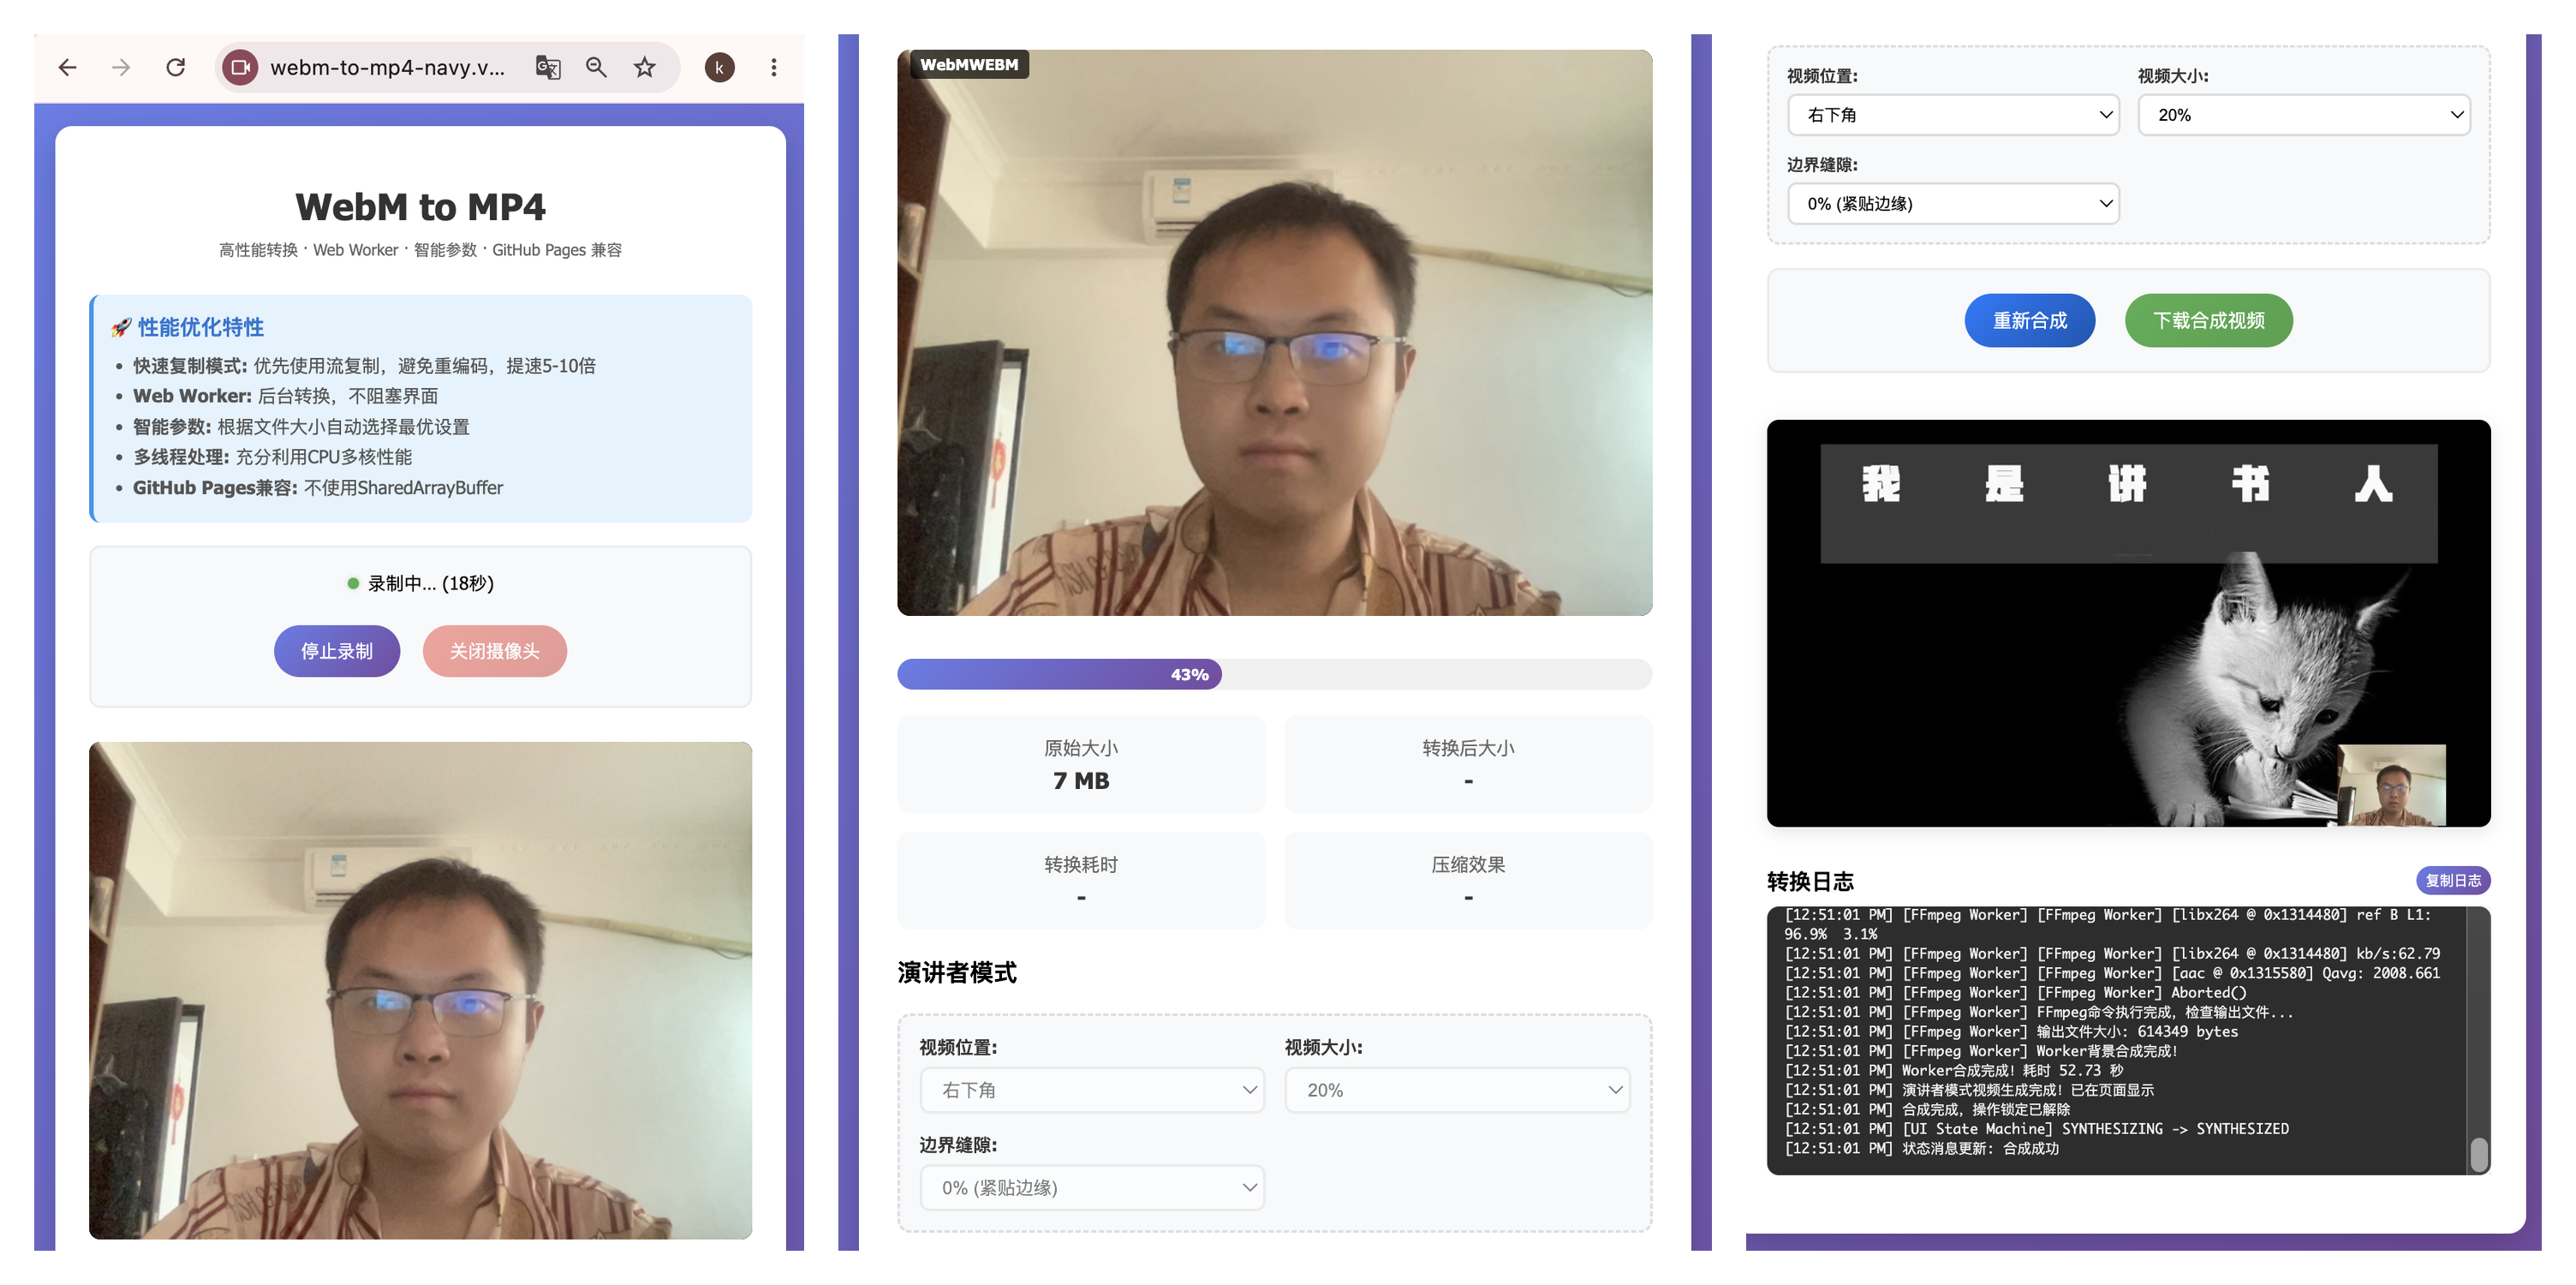
\includegraphics[width=1.0\textwidth]{assets/01_teaser_teaser.png}
   \captionof{figure}{ Teaser: (a) Real-Time WebM Recording. Shows the active browser MediaRecorder session managing streams safely. (b) WASM MP4 Transcoding. Demonstrates the statistics of the Web Worker converting the video locally. (c) Client-Side Speaker Compositing. Displays the final HTML5 Canvas merging the presenter's video with background slides. }
   \label{fig:teaser}
\end{center}

}
\makeatother
\maketitle
\begin{abstract}
As web applications increasingly rely on rich media capture, the disparity between browser-native recording formats (e.g., WebM) and universally supported playback formats (e.g., MP4) presents a significant challenge. Traditional server-side transcoding architectures introduce high latency, bandwidth overhead, and complex infrastructure maintenance. This report introduces an entirely client-side framework that leverages WebAssembly (WASM) and Web Workers to perform high-performance video transcoding directly within the user's browser. By encapsulating FFmpeg operations in a non-blocking worker thread, the system ensures a fluid user interface while achieving near-native conversion speeds. Furthermore, we implement a novel "Speaker Mode" synthesis pipeline that dynamically composites the recorded video with presentation slides using HTML5 Canvas APIs, all managed by a robust, CSS-driven state machine. This zero-infrastructure approach not only eliminates server costs but also enhances user privacy by keeping all media processing strictly local.
\end{abstract}

% [BEGIN_BLOCK: 01_teaser]


% [END_BLOCK: 01_teaser]

% [BEGIN_BLOCK: 02_figure]
\begin{figure*}[t]
\begin{center}
   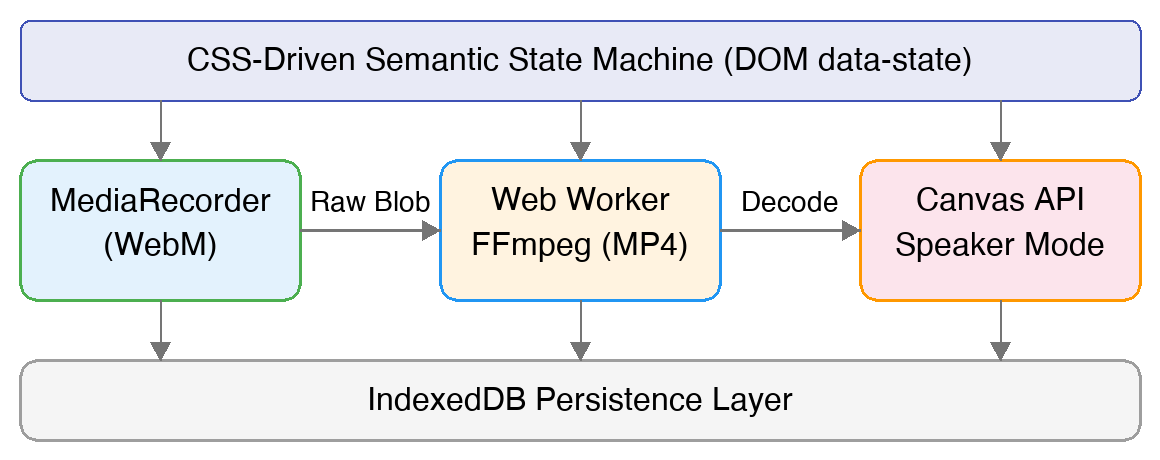
\includegraphics[width=1.0\linewidth]{assets/02_figure_0_pipeline_flow.png}
\end{center}
   \caption{Architecture of the client-side serverless integration pipeline. The CSS-driven semantic state machine orchestrates the entire lifecycle: directing the MediaRecorder, initiating the Web Worker FFmpeg transcoding, and finally driving the Canvas API for Speaker Mode compositing. All critical assets are asynchronously persisted to the IndexedDB layer to guarantee data safety across page unloads.}
   \label{fig:pipeline}
\end{figure*}
% [END_BLOCK: 02_figure]

% [BEGIN_BLOCK: 03_section]
\section{Introduction}

% [BEGIN_BLOCK: 01_text]
The widespread adoption of the MediaRecorder API has enabled modern browsers to seamlessly capture audio and video streams. However, these recordings are predominantly encoded in the WebM format (using VP8/VP9 codecs), which suffers from limited compatibility across certain platforms and devices, particularly within the Apple ecosystem. To bridge this gap, developers have historically relied on uploading raw WebM blobs to centralized backend servers running FFmpeg for transcoding to the ubiquitous MP4 (H.264) format. This server-side paradigm introduces substantial friction: users must endure upload wait times, applications consume massive bandwidth, and service providers incur significant computational costs to maintain scalable video processing infrastructure.

In this work, we present a paradigm shift towards decentralized, edge-computing video processing. By integrating an optimized WebAssembly compilation of FFmpeg, our framework executes complex transcoding pipelines directly within the client's browser. We mitigate the CPU-intensive nature of this task by isolating the FFmpeg core within a dedicated Web Worker, preventing main-thread blocking and preserving UI responsiveness. Beyond simple format conversion, we extend the client-side capabilities to include dynamic video compositing. Our "Speaker Mode" feature allows users to instantly superimpose their webcam recording onto presentation slides, generating professional-grade instructional videos without leaving the webpage.

% [END_BLOCK: 01_text]

% [END_BLOCK: 03_section]

% [BEGIN_BLOCK: 04_section]
\section{System Architecture}

% [BEGIN_BLOCK: 01_text]
Our framework is fundamentally divided into three synergistic components: a robust media capture and persistence layer, a multi-threaded WASM transcoding engine, and a declarative UI state manager (see Figure \ref{fig:pipeline}).

% [END_BLOCK: 01_text]

% [BEGIN_BLOCK: 02_text]
The entire application lifecycle is orchestrated by a rigorous, CSS-driven semantic state machine, ensuring predictable behavior and rapid development iteration without the entropy of imperative UI updates.

% [END_BLOCK: 02_text]

% [BEGIN_BLOCK: 03_subsection]
\subsection{Media Capture and Persistence}

% [BEGIN_BLOCK: 01_text]
The system initializes by securing media streams via the \texttt{navigator.mediaDevices.getUserMedia} API. The resulting \texttt{MediaRecorder} generates sequential WebM blobs. Recognizing the volatile nature of in-memory data, especially for large media files, we implemented an IndexedDB-based persistence layer.

Both the raw WebM and the transcoded MP4 (as well as the synthesized Speaker Mode video) are continuously committed to local storage, indexed by unique session IDs. This ensures that users can refresh the application or return later without losing computational progress, a crucial requirement for client-side heavy workloads.

Listing~\ref{lst:persistence} illustrates the asynchronous IndexedDB transactions used to securely read and write gigabyte-scale video blobs directly within the browser's storage sandbox.

% [END_BLOCK: 01_text]

% [END_BLOCK: 03_subsection]

% [BEGIN_BLOCK: 04_code]
\begin{lstlisting}[language=java,breaklines=true,breakatwhitespace=true,basicstyle=\ttfamily\small,caption={Asynchronous IndexedDB transactions for large media blob persistence.},label={lst:persistence}]
async persistState() {
  const data = {
    webm: this.webmBlob,
    mp4: this.mp4Blob,
    speaker: this.speakerBlob,
    // ... metadata ...
  };
  await db.transaction('rw', db.sessions, async () => {
    await db.sessions.put({ id: this.sid, ...data });
  });
}
\end{lstlisting}

% [END_BLOCK: 04_code]

% [BEGIN_BLOCK: 05_subsection]
\subsection{Web Worker FFmpeg Pipeline}

% [BEGIN_BLOCK: 01_text]
The core of our performance optimization is the \texttt{OptimizedFFmpegConverter}. To avoid blocking the main thread during intensive H.264 encoding, the FFmpeg WASM module is instantiated entirely within a dedicated Web Worker. This addresses a critical limitation: standard FFmpeg WASM heavily relies on \texttt{SharedArrayBuffer} for multithreading, which mandates strict Cross-Origin Isolation (COOP/COEP) headers. To ensure compatibility with static hosts like GitHub Pages or Vercel, our pipeline utilizes a specialized single-threaded WASM build, optimizing encoding parameters (e.g., \texttt{-preset ultrafast}) to offset the lack of multithreading. Communication is handled via structured cloning of ArrayBuffers, ensuring memory safety and efficient transfer.

% [END_BLOCK: 01_text]

% [END_BLOCK: 05_subsection]

% [BEGIN_BLOCK: 06_figure]
\begin{figure}[htbp]
\begin{center}
   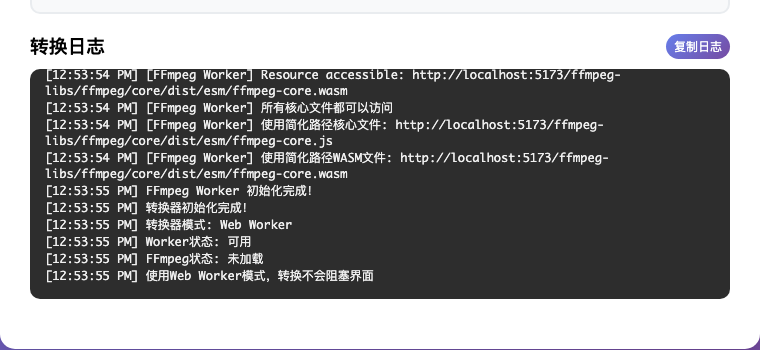
\includegraphics[width=1.0\linewidth]{assets/06_figure_0_fig_init.png}
\end{center}
   \caption{The initialization process. The system loads core libraries (e.g., FFmpeg WebAssembly modules) locally to ensure a self-contained execution environment before enabling capture.}
   \label{fig:init}
\end{figure}
% [END_BLOCK: 06_figure]

% [BEGIN_BLOCK: 07_subsection]
\subsection{CSS-Driven Semantic State Machine}

% [BEGIN_BLOCK: 01_text]
Managing asynchronous video operations introduces significant state entropy. To resolve this, we enforce a strict state machine pattern mapped directly to the DOM. Instead of imperatively toggling the visibility of individual buttons via JavaScript, the application state is maintained in a central store and propagated to the \texttt{body} tag as a \texttt{data-state} attribute (e.g., \texttt{INITIAL}, \texttt{RECORDING}, \texttt{CONVERTING}, \texttt{SYNTHESIZED}). A corresponding \texttt{state.css} file exclusively dictates the visibility (\texttt{display: none !important}) and interactability of all UI elements based on this root attribute. This declarative approach guarantees that the UI perfectly mirrors the internal logic, preventing invalid state transitions (e.g., attempting to download before conversion is complete).

% [END_BLOCK: 01_text]

% [END_BLOCK: 07_subsection]

% [END_BLOCK: 04_section]

% [BEGIN_BLOCK: 05_section]
\section{Interactive Video Compositing}

% [BEGIN_BLOCK: 01_text]
A novel contribution of this framework is the "Speaker Mode" feature, which demonstrates the feasibility of complex video editing tasks purely on the client side.

% [END_BLOCK: 01_text]

% [BEGIN_BLOCK: 02_subsection]
\subsection{FFmpeg-Based Video Compositing}

% [BEGIN_BLOCK: 01_text]
Upon completion of a recording, the system allows the user to superimpose their webcam footage onto a static presentation background. Rather than relying on the \texttt{MediaRecorder} API to capture an HTML5 Canvas stream---which often suffers from frame drops and encoding quality degradation---we offload the final synthesis entirely to the Web Worker FFmpeg pipeline.

% [END_BLOCK: 01_text]

% [BEGIN_BLOCK: 02_text]
The system utilizes FFmpeg's \texttt{overlay} and \texttt{scale} filters to composite the original high-quality WebM blob over the presentation slide in the background. The Canvas API is retained strictly as an interactive, real-time preview interface (see Figure \ref{fig:speaker}) to assist users in adjusting the position and scale of the video overlay before committing to the heavy FFmpeg computation.

% [END_BLOCK: 02_text]

% [END_BLOCK: 02_subsection]

% [BEGIN_BLOCK: 03_figure]
\begin{figure}[htbp]
\begin{center}
   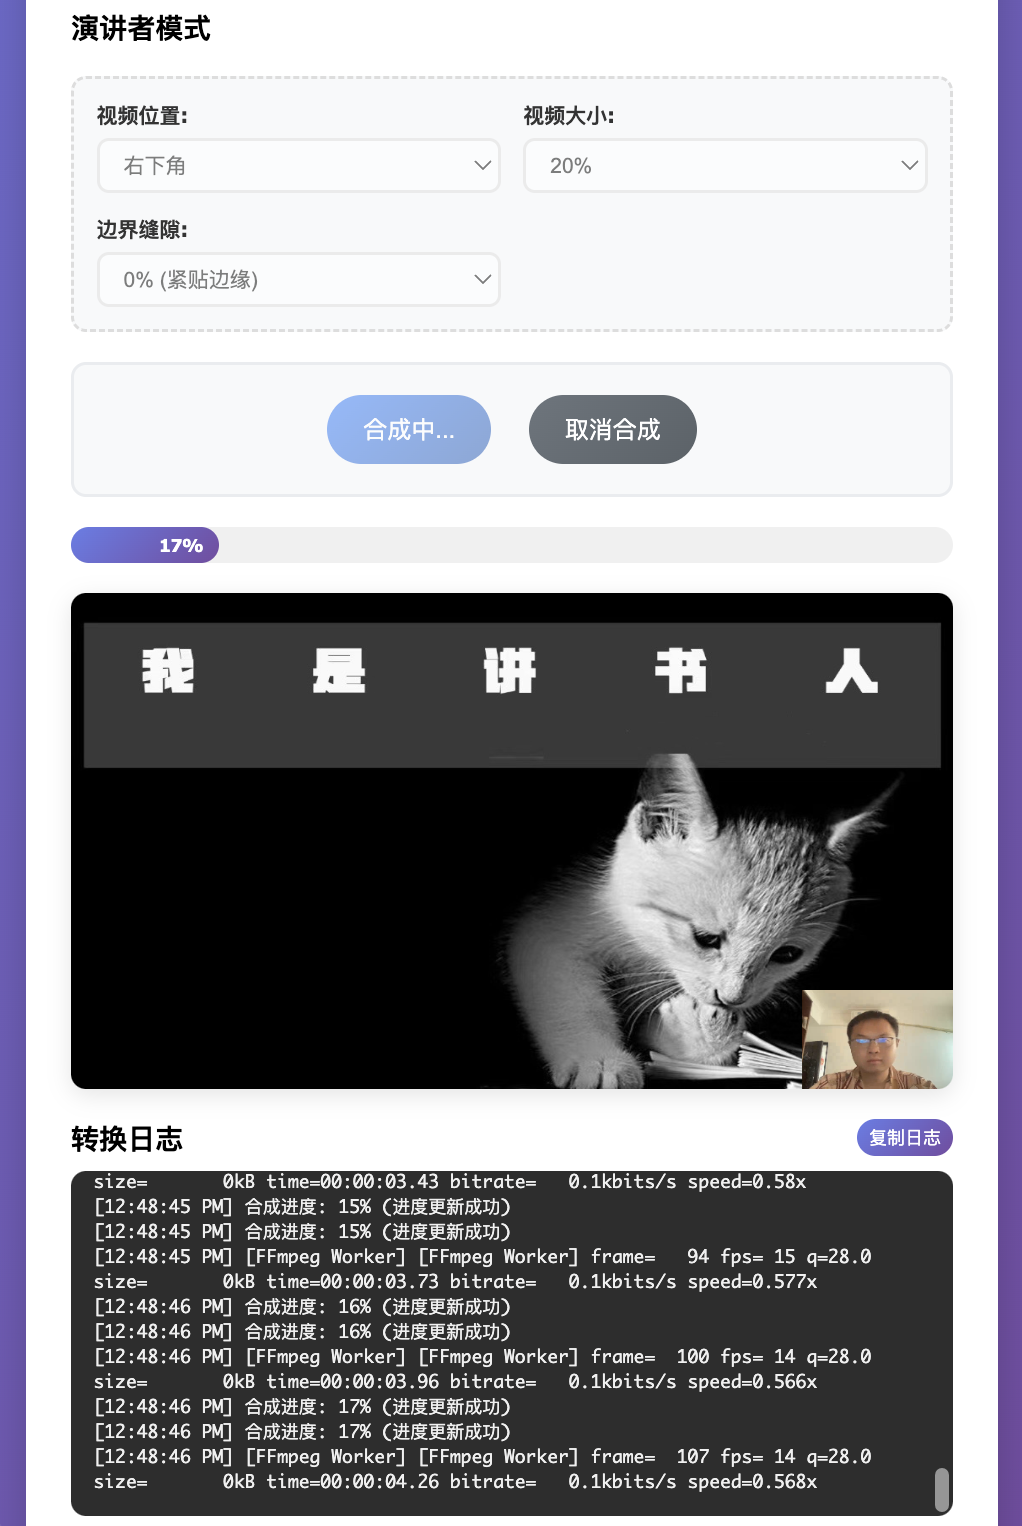
\includegraphics[width=1.0\linewidth]{assets/03_figure_0_fig_speaker.png}
\end{center}
   \caption{The Speaker Mode preview interface, capturing the exact moment the HTML5 Canvas draws the video frame before handing over the poster image to the target video element.}
   \label{fig:speaker}
\end{figure}
% [END_BLOCK: 03_figure]

% [BEGIN_BLOCK: 04_subsection]
\subsection{Resolving Rendering Race Conditions}

% [BEGIN_BLOCK: 01_text]
A significant technical hurdle in client-side video manipulation is managing the asynchronous lifecycle of dynamically generated Blob URLs. When restoring a session or immediately after rendering, the browser may not eagerly decode the first frame of a Blob video, resulting in a blank container. We solved this by implementing a ``CSS Stacking Handover'' protocol (see Listing \ref{lst:handover}).

% [END_BLOCK: 01_text]

% [BEGIN_BLOCK: 02_text]
The system forces the Canvas to explicitly draw the first composite frame and displays it as a fallback layer. The dynamically generated \texttt{<video>} element is placed directly above it. Once the video fires the \texttt{oncanplay} event, indicating the Blob is fully decoded and ready to paint, the underlying Canvas is hidden. This physical layering guarantees exact visual continuity and elegantly masks the ``black screen'' delay inherent in Chromium's Blob handling.

% [END_BLOCK: 02_text]

% [BEGIN_BLOCK: 03_code]
\begin{lstlisting}[language=java,breaklines=true,breakatwhitespace=true,basicstyle=\ttfamily\small,caption={CSS Stacking Handover logic for visual continuity.},label={lst:handover}]
const speakerVideo = document.createElement('video');
speakerVideo.src = downloadUrl; // Blob URL from FFmpeg
speakerVideo.className = 'speaker-video';

// Hide fallback Canvas only when video is ready to paint
speakerVideo.oncanplay = () => {
    elements.speakerCanvas.style.display = 'none';
};
elements.speakerPreview.appendChild(speakerVideo);
\end{lstlisting}

% [END_BLOCK: 03_code]

% [END_BLOCK: 04_subsection]

% [END_BLOCK: 05_section]

% [BEGIN_BLOCK: 06_section]
\section{Conclusion and Future Work}

% [BEGIN_BLOCK: 01_text]
We have demonstrated a robust, purely client-side architecture for video recording, FFmpeg-based transcoding, and dynamic video synthesis. By leveraging Web Workers and a strict CSS-driven state machine, the framework delivers server-equivalent functionality with zero backend infrastructure, ensuring high performance, low latency, and absolute data privacy. Future work will focus on integrating this offline video processing engine with localized Large Language Models (LLMs) via WebGPU, enabling entirely client-side transcription, summarization, and automated editing of the recorded presentations.

% [END_BLOCK: 01_text]

% [END_BLOCK: 06_section]

\end{document}